There are five major steps in our methodology(Figure~\ref{fig:tool_flow}).
First, the \emph{signal selection} step walks the circuit graph in FIRRTL\cite{Li:EECS-2016-9}
and picks important signal candidates according to the circuit topology. 
Next, the \emph{power model construct and training} step builds a power model 
using selected signals and trains the model using preliminary
waveforms from small workloads. The \emph{RTL instrumentation} step automatically
instrument FPGA performance simulators generated by Strober~\cite{Kim2016} with 
the activity counters for the signals from the previous step. 
The \emph{power prediction} step computes the power dissipation in real time
during FPGA performance simulation. Finally, the \emph{power validation} step
validates the power model by comparing against the power estimation from Strober,
and further trains the power model if necessary.

\begin{figure}[!ht]
	\centering
	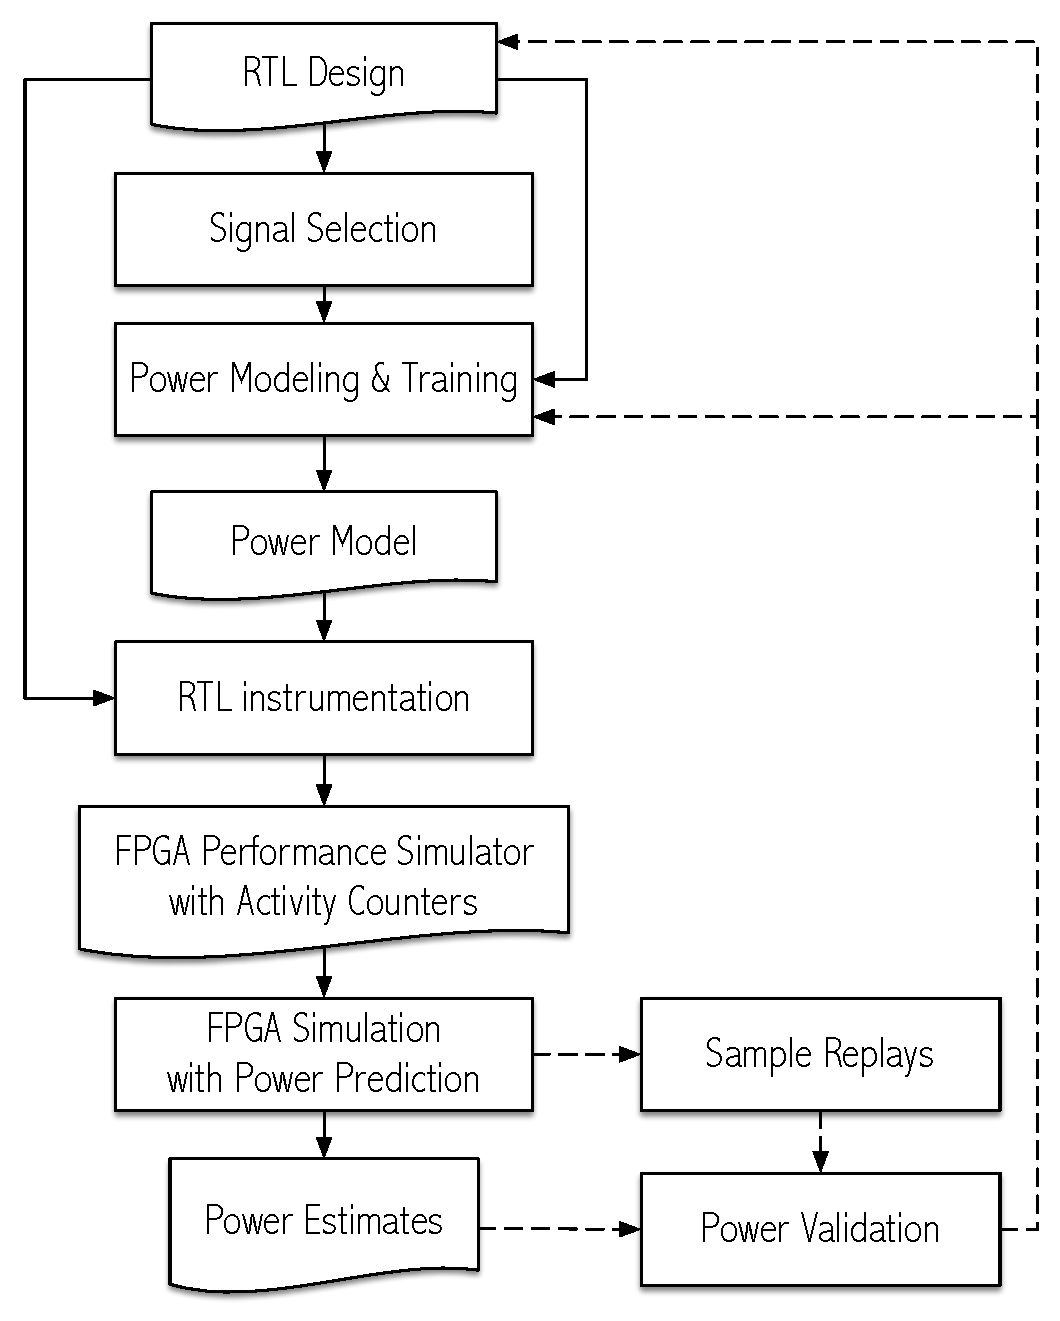
\includegraphics[width=0.4\textwidth,height=\textheight,keepaspectratio]{images/tool_flow.pdf}
	\caption{Overall Tool Flow}
	\label{fig:tool_flow}
\end{figure}

\subsection{Signal Selection}
\label{sec:signal_selection}
To construct and train a power model, we should select a subset of signals
because it is infeasible to keep track of all signal activities on the FPGA.
Firgure~\ref{fig:signal_selection} describes how power sensitive signals
are selected.

First of all, a random RTL design is fed into the FIRRTL compiler.
In this paper, we assume this design is written with Chisel~\cite{Bachrach2012}.
However, the target designs are not necessarily developed with Chisel
because the FIRRTL compiler will support various languages including Verilog in the near future.

In the FIRRTL compiler, a circuit graph is expressed with an intermediate representation,
FIRRTL~\cite{Li:EECS-2016-9}, so that a designer can write custom compiler passes for their
design. In this step, a custom pass selecting important signals and dumping the signal list
is implemented. The output signal list will be passed to the next step to build
a design-specific power model.

\begin{figure}[!ht]
	\centering
	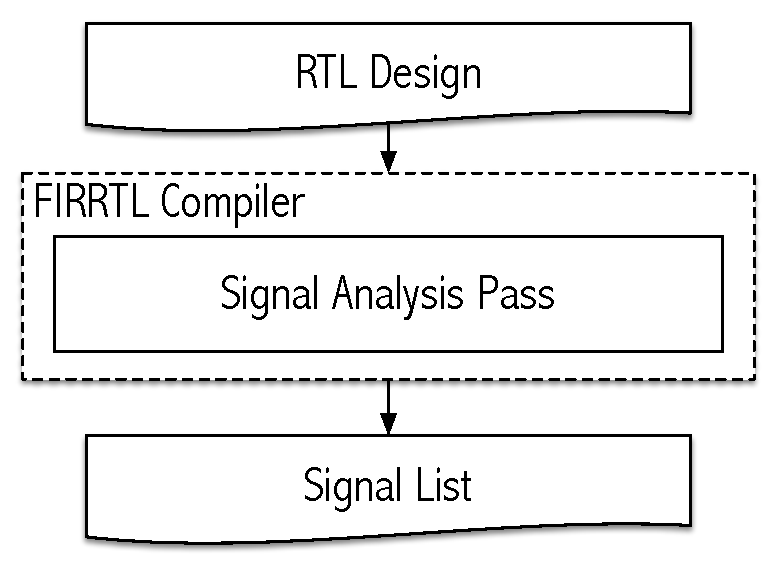
\includegraphics[width=0.35\textwidth,height=\textheight,keepaspectratio]{images/signal_selection.pdf}
	\caption{Signal Selection}
	\label{fig:signal_selection}
\end{figure}

\subsection{Power Modeling and Training}
\label{sec:power_modeling}
Once the signal list is obtained from the previous step, a design-specific power model can be
constructed expressed with the signal toggle activities in the list. Figure~\ref{fig:power_modeling}
explains how power models are built and trained. First, an RTL design is fed into the logic
synthesis tool(e.g. Synopsys Design Compiler~\textregistered) and the place-and-route tool
(e.g. Synopsys IC Compiler~\textregistered) to obtain a gate-level design, which is simulated
in SDF back-annotated gate-level simulation(e.g. Synopsys VCS~\textregistered) for accurate power estimates
by the power analysis tool(e.g. Synopsys PrimeTime PX~\textregistered).

RTL signal activities are also computed from RTL simulation(e.g. Verilator, Synopsys VCS~\textregistered).
By providing the signal list, the RTL signal activities, and the detailed power estimates
to the power modeling and training algorithm, a design-specific power model can be constructed
expressed with the signal toggle activities.

For RTL simulation and gate-level simulation, microbenchmarks or random instruction streams are employed
for initial power model training. In addition, there can be random execution sample snapshots from
long-running FPGA performance simulation~\cite{Kim2016}, which are used not only for power model validation
but also for further training the power model for more accurate power estimates.

\begin{figure}[!ht]
	\centering
	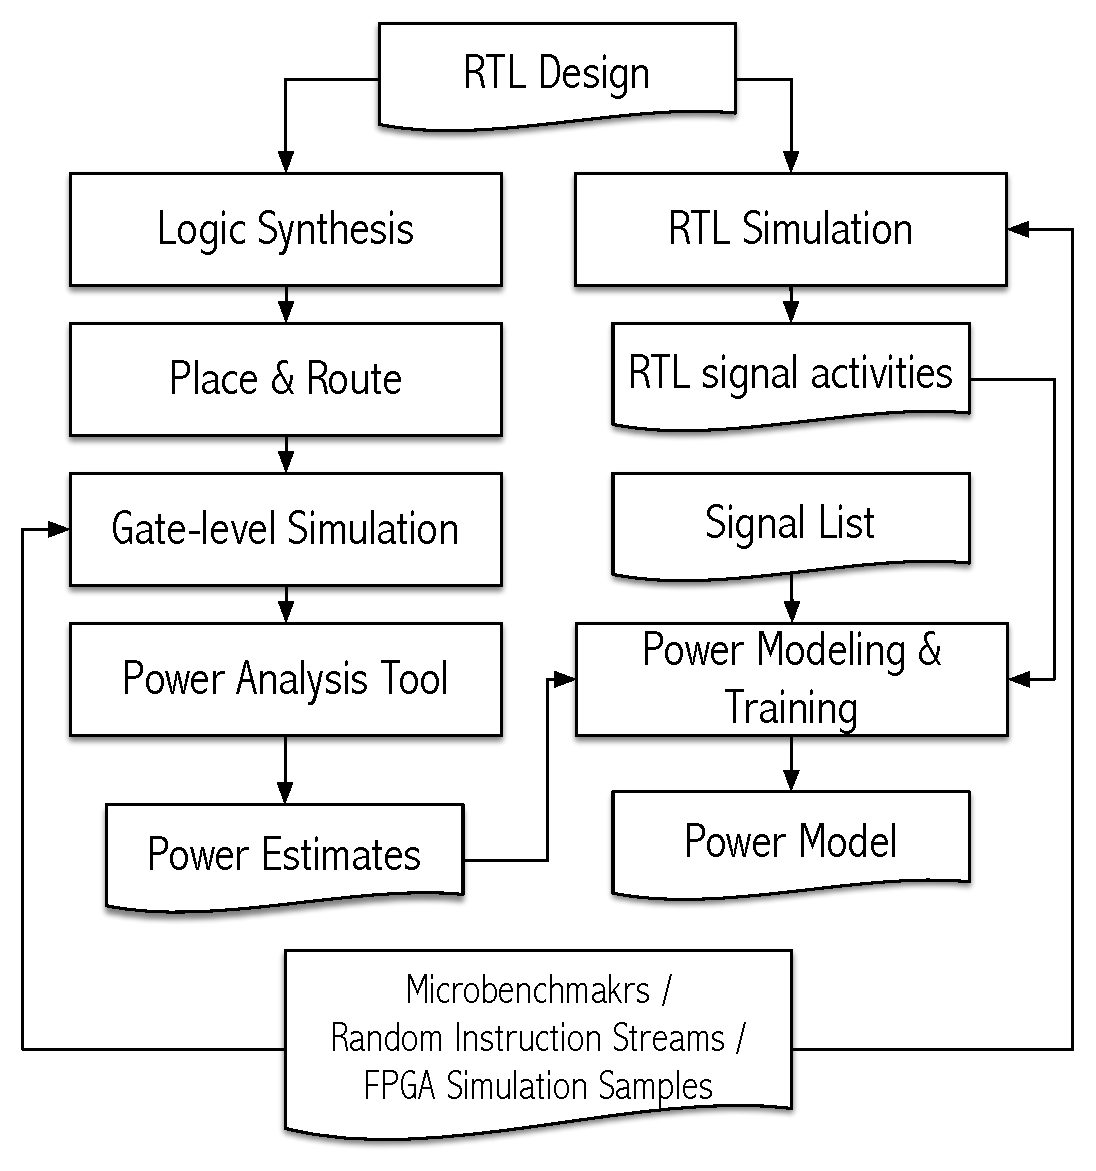
\includegraphics[width=0.4\textwidth,height=\textheight,keepaspectratio]{images/power_modeling.pdf}
	\caption{Power Modeling and Training}
	\label{fig:power_modeling}
\end{figure}

\subsubsection{Macromodels for Complex Combinational Logic}
Previous work~\cite{Sunwoo2010} suggests that linear power models for complex combinational logic such as ALUs, SEC/DED circuits, interrupt controllers, and multipliers are inaccurate. To overcome this issue, we turn to macromodels which attempt to estimate the power of complex logic by only looking at the input and output switching activity of the combinational block. In this paper we will measure the accuracy of a previously proposed power macromodel that uses 4 statistics $P_{in}, D_{in}, SC_{in}, D_{out}$.~\cite{Najm2000}\cite{Najm2000_2}

This macromodel considers sequences of input vectors into a combinational block. Each sequence may contain $N$ input vectors. Then we can define for a given sequence,
\begin{itemize}
	\item $P_{in}$ = average number of input bits that are logic 1 across a sequence
	\item $D_{in}$ = average number of input bit transitions across a sequence (average input transition density)
	\item $SC_{in}$ = average spacial correlation coefficient across a sequence and across all input bit pairs
	\item $D_{out}$ = average number of output bit transitions across a sequence (average output transition density)
\end{itemize}

We will generate multiple sequences of input training vectors, derive an accurate power estimate from PrimeTime, and use the computed statistics above to train the macromodel. We will then generate a separate set of sequences which will be used to test the macromodel's accuracy as compared to the PrimeTime power estimate.

\subsection{RTL Instrumentation}
\label{sec:instrumentation}
The RTL instrumentation is built upon the Chisel3 and FIRRTL port of the Strober's flow
to generate FPGA performance simulators. Figure~\ref{fig:power_modeling} shows how
the FPGA performance simulators are instrumented with the signal activity counters.

First, the target RTL design is FAME1-transformed to create the FPGA performance simulator~\cite{Kim2016}
in the FIRRTL compiler. Then, a custom transform is executed to attach activity counters
to the FPGA performance simulator by using the signal list from Section~\ref{sec:signal_selection}.
In addition, scan chains are inserted not only to read out the activity counter values but also to
capture RTL state snapshots to validate the power model. Finally, simulation mapping and platform mapping
are conducted for FPGA simulation~\cite{Kim2016}.

Note that signal selection in Section~\ref{sec:signal_selection} can be integrated to
this flow if signals are not pruned during power modeling and training in
Section~\ref{sec:power_modeling}. In this case, FPGA simulation can run in parallel while
training power models, which uses slow CAD tools extensively.

\begin{figure}[!ht]
	\centering
	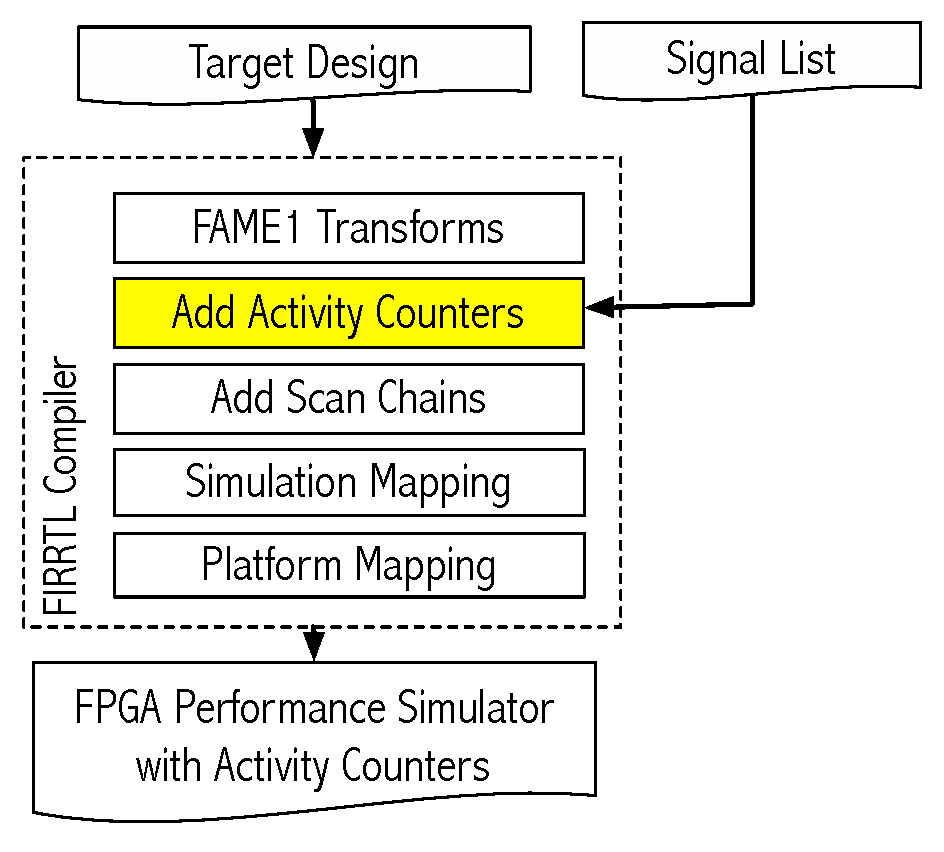
\includegraphics[width=0.4\textwidth,height=\textheight,keepaspectratio]{images/instrumentation.pdf}
	\caption{Power Modeling and Training}
	\label{fig:power_modeling}
\end{figure}

\subsection{Power Prediction during FPGA Simulation}
\label{sec:power_prediction}
Once the FPGA performance simulator instrumented with activity counters is obtained,
power estimates are quickly available during FPGA simulation. Since the target RTL
is FAME1-transformed, FPGA simulation can be easily paused, and activity counter
values are read out from the FPGA in the same way random RTL state sample snapnots
are taken in Strober~\cite{Kim2016}. If the power model is not available during
FPGA simulation because it is still trained, the activity counter values are saved
to estimate the power dissipation later.

\subsection{Power Validation}
\label{sec:power_validation}
Designers may want to validate the power estimates from Section~\ref{sec:power_prediction}
after FPGA simulation. Since this methodology is combined with Strober,
an accurate power estimates with statistically bounded errors are available by
replaying random RTL state snapshots, which are used to further train the power model
for more accurate power estimates (Figure~\ref{fig:power_modeling}).
